% --------------------------------------------------------------
% This is all preamble stuff that you don't have to worry about.
% Head down to where it says "Start here"
% --------------------------------------------------------------
\documentclass[12pt]{article}
\usepackage[top=2cm,bottom=2cm,left=2.5cm,right=3cm,headsep=8pt,a4paper]{geometry}
\usepackage{listings}
\usepackage[usenames]{color}
\definecolor{gray97}{gray}{.97}
\definecolor{gray75}{gray}{.75}
\definecolor{gray45}{gray}{.45}
\definecolor{azul1}{RGB}{141,198,163}
\definecolor{azul2}{RGB}{24,107,122}
\definecolor{verde1}{RGB}{44,186,34}
\usepackage{textcomp}
\lstset{
        frame=Ltb,
        framerule=1pt,
        framextopmargin=3pt,
        framexbottommargin=3pt,
        framexleftmargin=0.4cm,
        framesep=0pt,
        rulesep=.4pt,
		backgroundcolor=\color{gray97},
		rulesepcolor=,
        tabsize=4,
        rulecolor=\color[RGB]{106, 182, 217}, %AZUL
        upquote=true,
        aboveskip={1.5\baselineskip}, %despues de la linea de texto
        columns=fixed,
        showstringspaces=false,
        extendedchars=true,
        breaklines=true,
        prebreak = \raisebox{0ex}[0ex][0ex]{\ensuremath{\hookleftarrow}},
        showtabs=false,
        showspaces=false,
        showstringspaces=false,
        basicstyle=\scriptsize\ttfamily\color[RGB]{39, 100, 46}, %Numeros de lineas, simbolos, puntos y coma y demas
        identifierstyle=\ttfamily\color[RGB]{56, 140, 189}, %variables
        commentstyle=\color[RGB]{62, 179, 101}, %comentarios
        stringstyle=\color[RGB]{247, 165, 42}, %impresiones
        keywordstyle=\bfseries\color[RGB]{237, 118, 150}, %funciones
        %
		numbers=left,
		numbersep=5pt,
		numberstyle=\tiny,
		numberfirstline = false,
		breaklines=true,
		}
\usepackage{amsmath,amsthm,amssymb}
\usepackage[spanish]{babel} %Castellanización
\usepackage[T1]{fontenc} %escribe lo del teclado
\usepackage[utf8]{inputenc} %Reconoce algunos símbolos
\usepackage{lmodern} %optimiza algunas fuentes
\usepackage{graphicx}
\graphicspath{ {images/} }
\usepackage{hyperref} % Uso de links

\newcommand{\N}{\mathbb{N}}
\newcommand{\Z}{\mathbb{Z}}

\newenvironment{theorem}[2][Theorem]{\begin{trivlist}
\item[\hskip \labelsep {\bfseries #1}\hskip \labelsep {\bfseries #2.}]}{\end{trivlist}}
\newenvironment{lemma}[2][Lemma]{\begin{trivlist}
\item[\hskip \labelsep {\bfseries #1}\hskip \labelsep {\bfseries #2.}]}{\end{trivlist}}
\newenvironment{exercise}[2][Exercise]{\begin{trivlist}
\item[\hskip \labelsep {\bfseries #1}\hskip \labelsep {\bfseries #2.}]}{\end{trivlist}}
\newenvironment{problem}[2][Problem]{\begin{trivlist}
\item[\hskip \labelsep {\bfseries #1}\hskip \labelsep {\bfseries #2.}]}{\end{trivlist}}
\newenvironment{question}[2][Question]{\begin{trivlist}
\item[\hskip \labelsep {\bfseries #1}\hskip \labelsep {\bfseries #2.}]}{\end{trivlist}}
\newenvironment{corollary}[2][Corollary]{\begin{trivlist}
\item[\hskip \labelsep {\bfseries #1}\hskip \labelsep {\bfseries #2.}]}{\end{trivlist}}

\newenvironment{solution}{\begin{proof}[Solution]}{\end{proof}}
\begin{document}
% --------------------------------------------------------------
%                         Start here
% --------------------------------------------------------------
\title{Tarea 10}
\author{Hanan Ronaldo Quispe Condori\\ %replace with your name
Procesamiento de Señales II}

\maketitle
\section{Diseñar un filtro IIR utilizando fdatool, filtro pasabajas Chevyshev 1 (rizado banda de paso), $fc=1200Hz,fr=2300Hz,Ap=2dB,Ar=50dB$.}

En la herramienta de $fdatool$, se ingresaron las caracteristicas deseadas del filtro como se indica en la siguiente figura.
\begin{figure}[h]
    \centering
    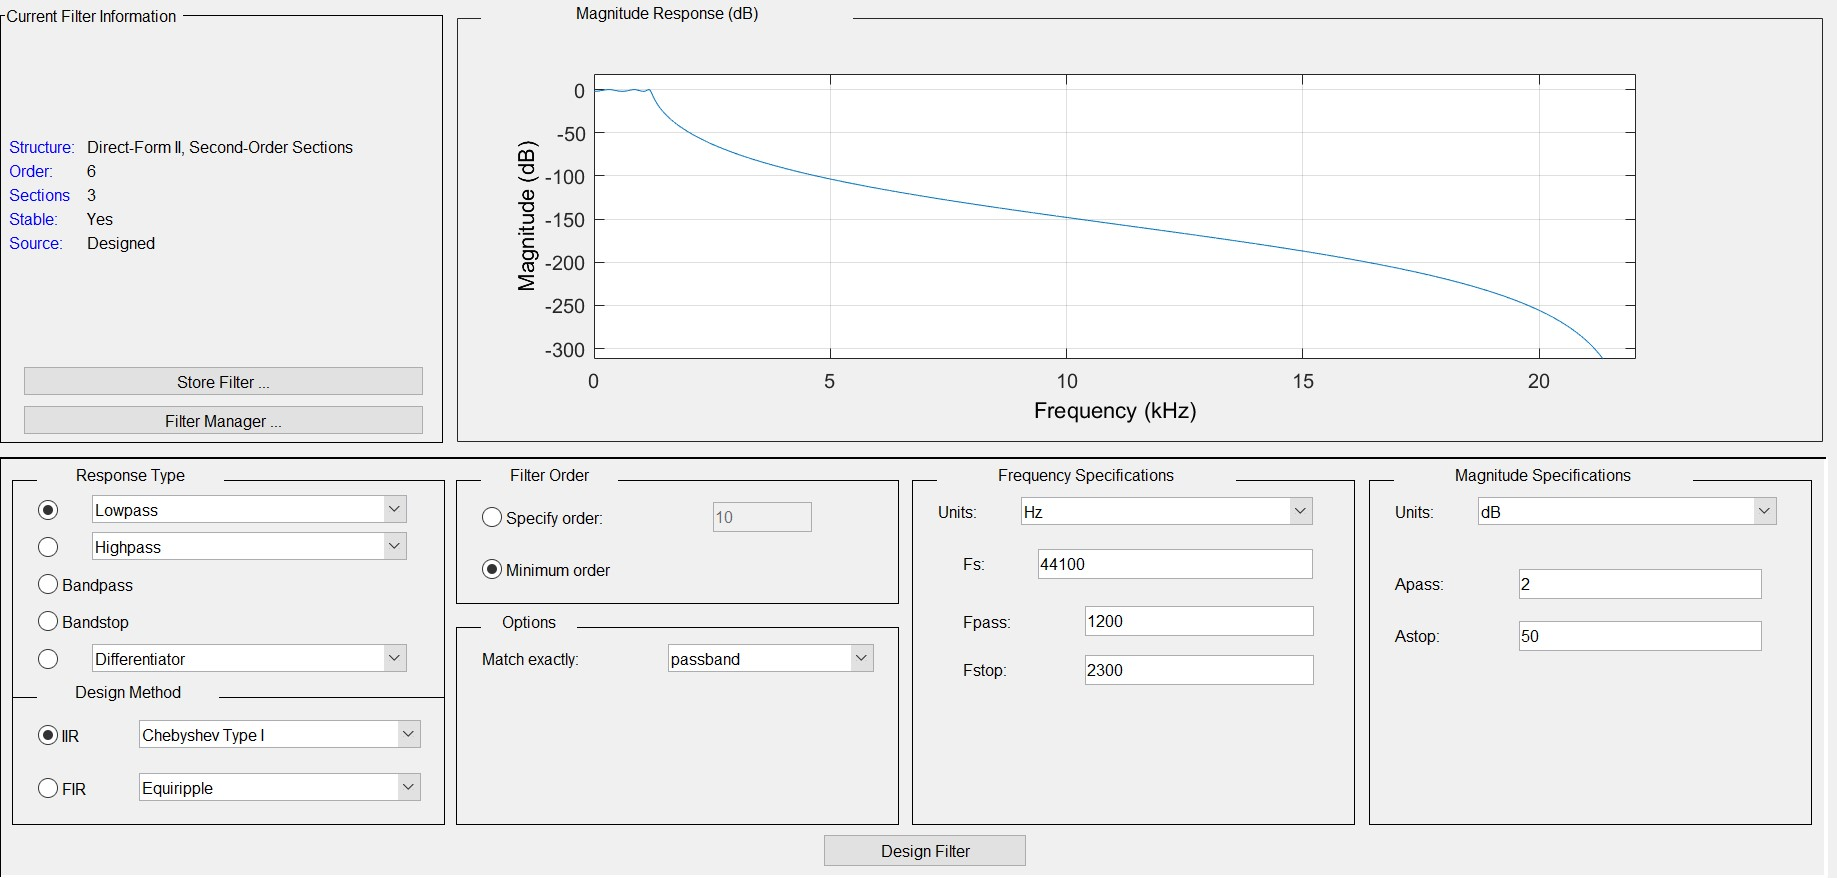
\includegraphics[width=15cm, height=8cm]{imagenes/fdatool.jpg}
    \caption{Interfaz Gráfica fdatool.}
    \label{fig:fda}
\end{figure}

Al exportar los resultados se obtuvo lo siguiente.
\lstinputlisting[language=matlab]{IIR_filter.fcf}

Del resultado podemos extraer la matriz SOS en la variable $"sos"$ para su conversión a función de transferencia, esto se realizara mediante la función $sos2tf$  como se muestra a continuación.

\lstinputlisting[language=matlab]{uso_ss2tf.m}

Como resultado se tienen los coeficientes de la función de transferencia del filtro.

\lstinputlisting[language=matlab]{result_sos2tf}

Una vez con estos valores se puede usar la función $freqz$ para obtener la respuesta en frecuencia del filtro diseñado.

\lstinputlisting[language=matlab]{uso_freqz.m}

Esta función da como resultado la siguiente gráfica de respuesta en frecuencia.

\begin{figure}[h]
    \centering
    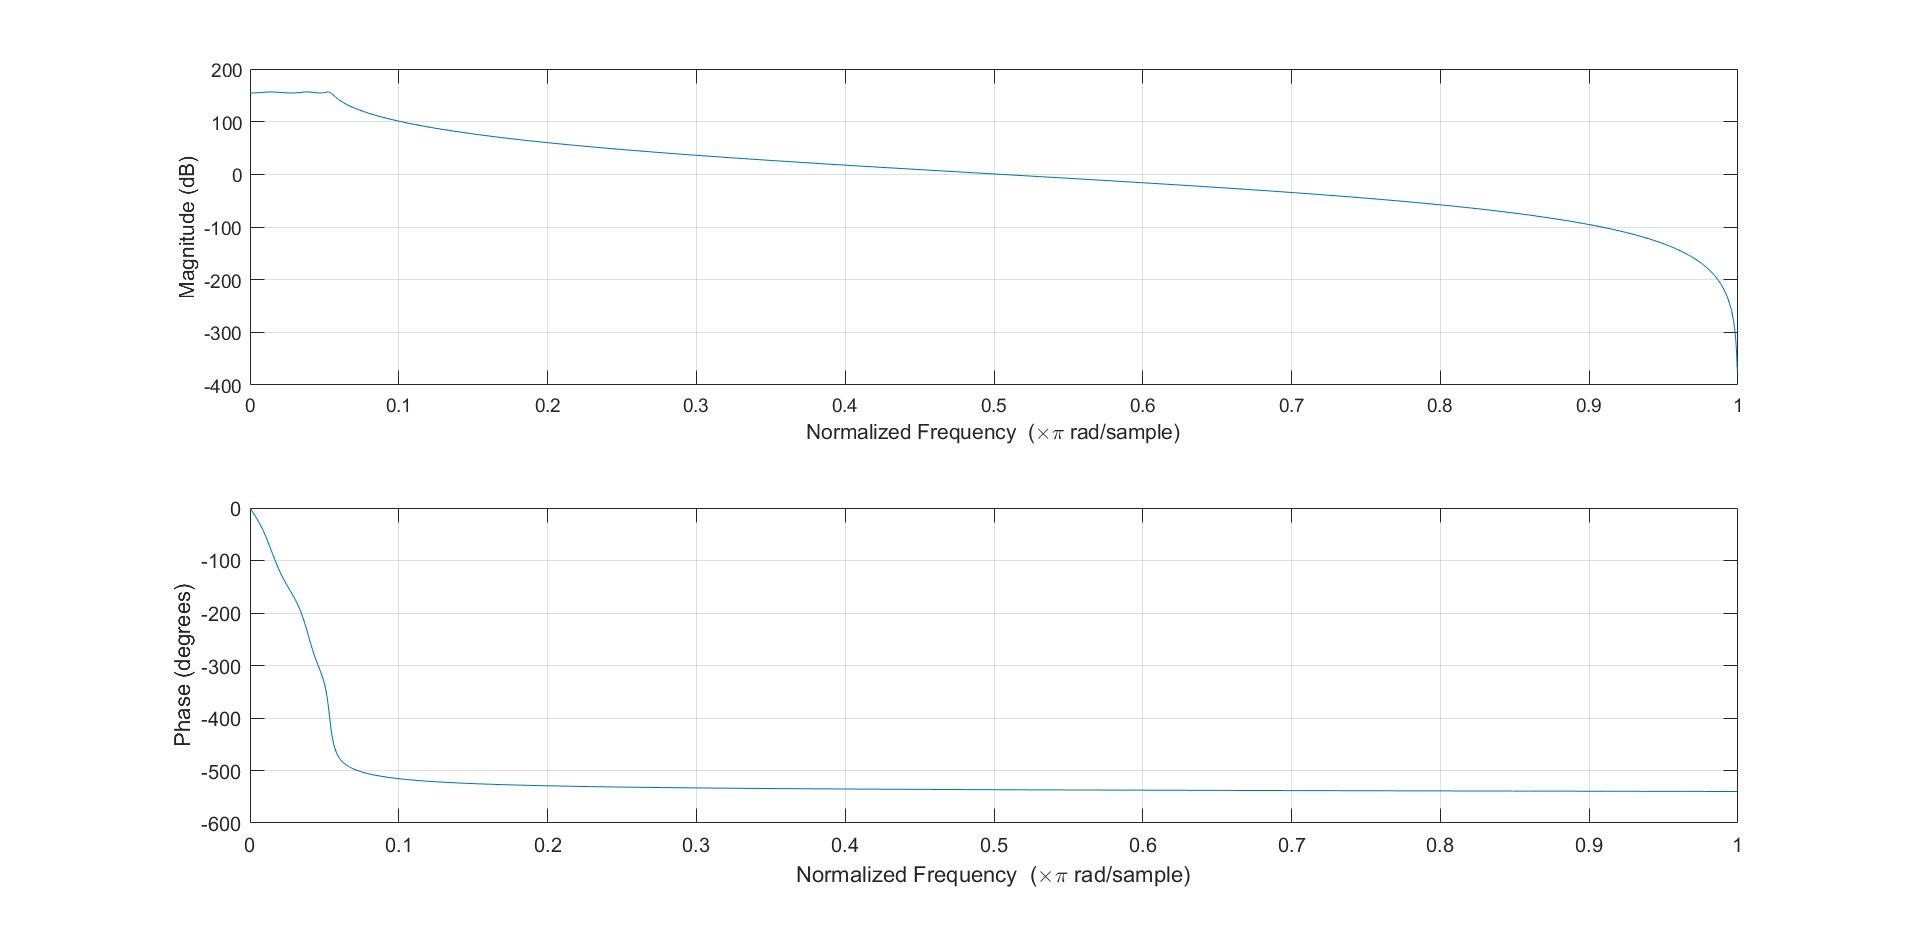
\includegraphics[width=15cm, height=8cm]{imagenes/result.jpg}
    \caption{Interfaz Gráfica fdatool.}
    \label{fig:fda}
\end{figure}
\end{document}